


In this section, we develop an algorithm that converges to a stationary point of the bilevel problem ({\it i.e.,} a stationary point of $F(x) = f(x,y^*(x))$) and makes use only of gradients of $f$ and $g$. 
Recall the  equivalent formulation \eqref{problem:penalty_bilevel}. 
To see how we can avoid second-order derivatives, we observe the gradient of $\grad \mL_{\lambda}$:
\begin{align*}
    \grad_x \mL_{\lambda}(x,y) &= \grad_x f(x,y) + \lambda (\grad_x g(x,y) - \grad g^*(x)), \\
    \grad_y \mL_{\lambda}(x,y) &= \grad_y f(x,y) + \lambda \grad_y g(x,y).
\end{align*}
Note that
\begin{align*}
    \grad g^*(x) &= \grad_x g(x,y^*(x)) + \grad_x y^*(x) \grad_y g(x, y^*(x)) = \grad_x g(x,y^*(x)),
\end{align*}
due to the optimality condition for $g$ at $y^*(x)$. 
Thus, we could consider optimizing $\mL_{\lambda} (x,y)$ by introducing an auxiliary variable $z$ that chases $y^*(x)$, and setting up an alternative bilevel formulation \eqref{problem:bilevel} with outer-level objective $\mL_{\lambda}(x', z)$, outer variable $x' = (x,y)$, and inner variable $z$. 
However, such an approach settles in a different landscape from that of  $F(x)$, resulting in a bias. 
The question is how tightly we can control this bias without compromising too much smoothness of the alternative function $\mL_{\lambda}$, which affects the overall step-size design and noise variance. 

%\swcomment{I'm not actually sure if this is best thought of as a Lagrangian, or as a nonsmooth penalty function (which penalizes the constraint violation). Both perspectives are problematic because of the degeneracy of the constraint in this formulation. Think about this more as the algorithm and analysis develop...}

To control the bias, we need a better understanding of how the functions $\mL_{\lambda}$ and $F(x)$ are related. 
Let us introduce an auxiliary function $\mL_{\lambda}^*$ defined as:
\begin{align*}
    \mL_{\lambda}^*(x) := \min_y \mL_\lambda (x,y).
\end{align*}
Note that if $\lambda > 2l_{f,1} / \mu_g$, then for every $\bar{x} \in X$, $\mL_{\lambda}(\bar{x},y)$ is at least $(\lambda \mu_g / 2)$ strongly-convex in $y$, and therefore its minimizer $y_{\lambda}^*(x)$ is uniquely well-defined:
\begin{align}
\label{eq:yls}
    y_{\lambda}^*(x) := \arg \min_y \mL_{\lambda} (x,y). 
\end{align}
Since $F(x) = \lim_{\lambda \rightarrow \infty} \mL_{\lambda}^*(x)$ for every $x \in X$, we could expect that $\mL_{\lambda}^*(x)$ is a well-defined proxy of $F(x)$ for sufficiently large $\lambda > 0$.
The following lemma confirms this intuition.
\begin{lemma}
    \label{lemma:l_star_lambda_approximate}
    For any $x \in X$ and $\lambda \ge 2l_{f,1} / \mu_g$, $\grad \mL_{\lambda}^*(x)$ is given by
    \begin{align*}
        \grad_x \mL_{\lambda} (x, y_{\lambda}^*(x)) &= \grad_x f(x,y_{\lambda}^*(x)) + \lambda (\grad_x g(x, y_{\lambda}^*(x)) - \grad_x g(x, y^*(x))).
    \end{align*}
    Furthermore,  we have
    \begin{align*}
        \| \grad F(x) - \grad \mL_\lambda^*(x) \| \le  C_\lambda / \lambda,
    \end{align*}
    where $C_\lambda := \frac{4 l_{f,0} l_{g,1}}{\mu_g^2} \left( l_{f,1} + \frac{2 l_{f,0} l_{g,2}}{\mu_g} \right)$. 
\end{lemma}
Importantly, $\grad \mL_{\lambda}^*(x)$ can be computed only with first-order derivatives of both $f$ and $g$. Thus any first-order method that finds a stationary point of $\mL_{\lambda}^*(x)$ approximately follows the trajectory of $x$ updated with the exact $\grad F(x)$, with a bias of $O(1/\lambda)$.


\begin{algorithm}[t]
    \caption{\algname}
    \label{algo:algo_name}
    
    {{\bf Input:} step sizes: $\{\alpha_k, \gamma_k\}$, multiplier difference sequence: $\{\delta_k\}$, inner-loop iteration count: $T$, step-size ratio: $\xi$, initializations: $\lambda_0, x_0, y_0, z_0$}
    \begin{algorithmic}[1]
        \FOR{$k = 0 ... K-1$}
            \STATE{$z_{k,0} \leftarrow z_{k}$, $y_{k,0} \leftarrow y_{k}$}
            \FOR{$t = 0 ... T-1$}
                \STATE{$z_{k,t+1} \leftarrow z_{k,t} - \gamma_k h_{gz}^{k,t}$}
                \STATE{$y_{k,t+1} \leftarrow y_{k,t} - \alpha_k (h_{fy}^{k,t} + \lambda_k h_{gy}^{k,t})$}
            \ENDFOR
            \STATE{$z_{k+1} \leftarrow z_{k,T}$, $y_{k+1} \leftarrow y_{k,T}$}
            \STATE{$x_{k+1} \leftarrow x_k - \xi \alpha_k (h_{fx}^k + \lambda_k (h_{gxy}^k - h_{gxz}^k))$}
            \STATE{$\lambda_{k+1} \leftarrow \lambda_k + \delta_k$}
        \ENDFOR
    \end{algorithmic}
\end{algorithm}

Our strategy is to use $\grad \mL_{\lambda}^*(x)$ as a proxy to $\grad F(x)$ for generating a sequence of iterates $\{x_k\}$. 
Accordingly, we introduce sequences $\{y_k\}$ and $\{z_k\}$ that approximate $y_{\lambda_k}^*(x_k)$ and $y^*(x_k)$, respectively. 
% Auxiliary sequences $y_k$ and $z_k$ are supposed to be good approximations of $y_{\lambda_k}^*(x_k)$ and $y^*(x_k)$ respectively, when we estimate $\grad \mL_{\lambda}^*(x)$. 
We gradually increase $\lambda_k$ with $k$, so that the bias in the sequence $\{x_k\}$ converges to 0. 



Our \textbf{F}ully \textbf{F}irst-order \textbf{S}tochastic \textbf{A}pproximation (\algname) method is shown in Algorithm \ref{algo:algo_name}. 
We emphasize that the method works with \emph{stochastic} gradients that are independent unbiased estimators of gradients, {\it i.e.,} 
\begin{align*}
    &h_{gz}^{k,t} := \nabla_y g(x_k, z_{k,t}; \phi_{z}^{k,t}), \ h_{fy}^{k,t} := \nabla_y f(x_k, y_{k,t}; \zeta_{y}^{k,t}), \\
    &h_{gy}^{k,t} := \nabla_y g(x_k, y_{k,t}; \phi_{y}^{k,t}), h_{gxy}^k:= \nabla_{x} g(x_k, y_{k+1}; \phi_{xy}^k), \\
    & h_{fx}^k := \nabla_x f(x_k, y_{k+1}; \zeta_{x}^k), h_{gxz}^k := \nabla_x g(x_k, z_{k+1}; \phi_{xz}^k).
\end{align*}
%This is in contrast to \cite{ye2022bome} that proposed a similar idea but only provided an algorithm for deterministic functions. Furthermore, we now only need the estimators of first-order derivatives of both $f$ and $g$, in contrast to most previous works that require the estimation of Jacobian or Hessian of $g$. 
The algorithm can set $T=1$ in conjunction with an appropriate choice of $\xi$, allowing a fully single-loop update for all variables. 





\subsection{Step-Size Design Principle} 
\label{sec:step}



We describe how we design the step-sizes for Algorithm \ref{algo:algo_name} to  achieve convergence to a $\epsilon$-stationary point of $F$. 
Several conditions must be satisfied. 
As will be shown in the analysis, with $(\lambda_k \mu_g/2)$-strong convexity of $\mL_{\lambda_k}$ in $y$, one-step inner iteration of $y_{k,t}$ is a contraction mapping toward $y_{\lambda,k}^*$ with rate $1 - O(\mu_g \beta_k)$. Henceforth, we often use the notatino $\beta_k := \alpha_k\lambda_k$, which is the effective step-size for updating $y_k$. 
For simplicity, we denote $y_{\lambda,k}^* := y_{\lambda_k}^* (x_k)$ and $y_k^* := y^*(x_k)$.  

We now describe the specific rules. First, essentially the step size we use for $x_k$ is $\xi \alpha_k$, and thus, $\alpha_k = \Omega(1/k)$ (otherwise, $\sum_k \alpha_k < \infty$, and $x_k$ fails to converge). 
On the other hand, since $\beta_k=\alpha_k\lambda_k$ is the effective step size for updating $y_k$, we need $\beta_k < O(1/l_{g,1}) = O(1)$. 
Together, these observations imply that the maximum rate of growth for $\lambda_k$ cannot exceed $O(k)$. 

Second, note that $\|x_{k+1} - x_k\|$ is (roughly) proportional to
\begin{align*}
    \|\grad F(x_k)\| + C_\lambda/\lambda_k + \lambda_k \|y_k - y_{\lambda, k}^*\| + \lambda_k \|z_k - y_{k}^*\|.
\end{align*}
This rate is optimized when $\|y_{k} - y_{\lambda,k}^*\| \asymp \|z_k - y_k^*\| \asymp \lambda_k^{-2}$. Thus, the ideal growth rate for $\lambda_k$ is $\|y_{k} - y_{\lambda,k}^*\|^{1/2}$ or $\|z_k - y_k^*\|^{1/2}$. 
We will design the rate of convergence of $y_k$ and $z_k$ to be the same, {\it i.e.,} $\beta_k \asymp \gamma_k$. 
For instance, when we have stochastic noises in the gradient estimate of $g$, {\it i.e.,} $\sigma_g^2 > 0$, the expected convergence rate of $\|y_k - y_{\lambda_k}^*\|^2$ is $O(\beta_k)$, since the sequence is optimized for strongly convex functions. 
This suggests $\lambda_k \asymp \beta_k^{-1/4}$ as the ideal rate of growth for $\lambda_k$.




\begin{figure}[t]
    \centering
    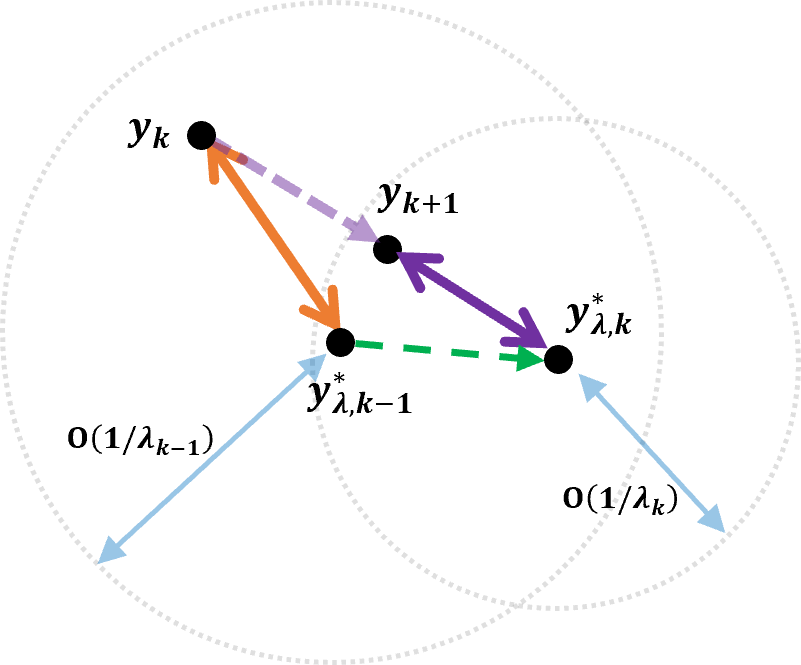
\includegraphics[width=0.4\textwidth]{Figures/contraction_picture.png}
    \caption{$y_k$ should move faster than $y_{\lambda_k}^*(x_k)$ moves, and stay within $O(1/\lambda_k)$-ball around $y_{\lambda_k}^*(x_k)$.}
    \label{fig:contraction_explain}
\end{figure}

The crux of Algorithm \ref{algo:algo_name} is how well $y_k$ (and $z_k$) can chase $y_{\lambda_k}^*(x_k)$ (resp. $y^*(x_k)$) when $x_k$ and $\lambda_k$ are changing  at every iteration. 
We characterize first how fast $y_\lambda^*(x)$ moves in relation to the movements of $\lambda$ and $x$.
%
\begin{lemma}
    \label{lemma:y_star_lagrangian_continuity}
    For any $x_1, x_2 \in X$ and for any $\lambda_2 \ge \lambda_1 \ge 2 l_{f,1} / \mu_g$, we have
    \begin{align*}
        \| y_{\lambda_1}^*(x_1) - y_{\lambda_2}^*(x_2)\| \le \frac{ 2(\lambda_2 - \lambda_1)}{\lambda_1\lambda_2} \frac{l_{f,0}}{\mu_g} + l_{\lambda,0} \|x_2 - x_1\|,
    \end{align*}
    for some $l_{\lambda,0} \le 3l_{g,1} / \mu_g$.
\end{lemma}
For Algorithm \ref{algo:algo_name} to converge to a desired point, $y_k$ should move sufficiently fast toward the current target $y_{\lambda,k}^*$ every iteration, dominating the movement of target $y_{\lambda, k}^*$ that results from updates to $x_k$ and $\lambda_k$ (see Figure~\ref{fig:contraction_explain}). 
At a minimum, the following condition should hold (in expectation):
\begin{align*}
    \|y_{k+1} - y_{\lambda, k}^*\| < \| y_k - y_{\lambda, k-1}^* \|.
\end{align*}


Since $\|y_{k+1} - y_{\lambda, k}^*\|^2$ can be bounded with $T$-steps of $1 - O(\mu_g \beta_k)$ contractions, starting from $y_k$, we require 
\begin{align*}
    \left(1 - O(T \mu_g \beta_k) \right) \|y_k - y_{\lambda, k}^*\|^2 < \|y_k - y_{\lambda, k-1}^*\|^2.
\end{align*}
Now, applying the bound in Lemma \ref{lemma:y_star_lagrangian_continuity}, the minimal condition is given by:
\begin{align*}
    \|y_{\lambda, k-1}^* - y_{\lambda,k}^*\| &\le (l_{f,0} / \mu_g) \cdot (\delta_k / \lambda_k^2) + l_{\lambda,0} \|x_{k} - x_{k-1}\| \le  T \mu_g \beta_k \| y_{k} - y_{\lambda, k-1}^* \|.
\end{align*}
Note that $\|y_{k+1} - y_{\lambda, k}^*\|$ should decay faster than $\lambda_k^{-1}$. Otherwise, the bias in updating $x_k$ using $y_k$ (to estimate $\grad \mL_{\lambda_k}^*$) is larger than $\lambda_k \|y_{k+1} - y_{\lambda,k}^*\|$, and this amount might blow up. Also, it can be easily seen that $\|x_{k} - x_{k-1}\| = \Omega(\xi \beta_k \|y_{k} - y_{\lambda,k-1}^*\|)$. 
We can thus derive two simple conditions:
\begin{align*}
    \frac{\delta_k}{\lambda_k} \le O_{\texttt{P}} (1) \cdot \beta_k, \ \frac{\xi}{T} < O_{\texttt{P}} (1),
\end{align*}
%\swcomment{What does the notation $O_{\texttt{P}}$ mean? Later $O_{\texttt{P}}(1)$ is defined to be an "instance-dependent constant." Perhaps define it here instead.} 
where $O_{\texttt{P}}(1)$ are instance-dependent constants. If $\lambda_k$ grows in some polynomial rate, then $\delta_k / \lambda_k = O(1/k)$ and the first condition is satisfied provided that $\beta_k = \Omega(1/k)$. 
The second condition indicates the number of inner iterations $T$ required for each outer iteration. 
We can set $T=1$ (thus making the algorithm single-loop) by setting $\xi$ sufficiently small.
Alternatively, we can set $\xi = 1$ choose $T>1$ to depend on some instance-specific parameters.


\subsection{Extension: Integrating Momentum}
\begin{algorithm}[t]
    \caption{\algnametwo}
    \label{algo:algo_name2}
    
    {{\bf Input:} step sizes: $\{\alpha_k, \gamma_k\}$, multiplier difference sequence: $\{\delta_k\}$, momentum-weight sequence $\{\eta_k\}$, step-size ratio: $\xi$, initialization: $\lambda_0, x_0, y_0, z_0$}
    \begin{algorithmic}[1]
        \FOR{$k = 0 ... K-1$}
            \STATE{$z_{k+1} \leftarrow z_{k} - \gamma_k \tilde{h}_{gz}^{k}$}
            \STATE{$y_{k+1} \leftarrow y_{k} - \alpha_k (\tilde{h}_{fy}^{k} + \lambda_k \tilde{h}_{gy}^{k})$}
            \STATE{$x_{k+1} \leftarrow x_k - \xi \alpha_k (\tilde{h}_{fx}^k + \lambda_k (\tilde{h}_{gxy}^k - \tilde{h}_{gxz}^k))$}
            \STATE{$\lambda_{k+1} \leftarrow \lambda_k + \delta_k$}
        \ENDFOR
    \end{algorithmic}
\end{algorithm}


Given the simple structure of Algorithm \ref{algo:algo_name}, we can integrate variance-reduction techniques to improve the overall convergence rates. 
One relevant technique is the momentum-assisting technique of \cite{khanduri2021near} for stochastic bilevel optimization. 
To simplify the presentation, we consider a fully single-loop variant by setting $T=1$. 

To apply the momentum technique, we only need to replace the simple unbiased gradient estimators $h$ with momentum-assisted gradient estimators $\tilde{h}$. 
For instance, $\tilde{h}_z^k$ can be defined with a proper momentum weight sequence $\eta_k \in (0,1]$ as follows:
\begin{align*}
    \tilde{h}_{z}^{k} := &\nabla_y g(x_k, z_{k}; \phi_{z}^{k}) + (1 - \eta_{k}) \left( \tilde{h}_{z}^{k-1} - \grad_y g(x_{k-1}, z_{k-1}; \phi_{z}^{k}) \right).
\end{align*}
Other quantities $\tilde{h}_{fy}$, $\tilde{h}_{gy}$, $\tilde{h}_{fx}$, $\tilde{h}_{gxy}$, $\tilde{h}_{gxz}$ are defined similarly, with the same momentum-weight sequence. 
We defer the full description of those quantities to Appendix~\ref{appendix:momentum_method}. 
The version of our algorithm that incorporates momentum is called \textbf{F}aster \textbf{F}ully \textbf{F}irst-order \textbf{S}tochastic \textbf{A}pproximation (\algnametwo); it is described in Algorithm~\ref{algo:algo_name2}, where we simply replace $h$ with $\tilde{h}$. 
Note that we have additional moment-weight parameters $\{\eta_{k}\}$.
% and we specify the details in Section \ref{section:analysis}. 






